\section{Manual de usuario}
\label{sec:manual}

\subsection{Página principal}

La página principal es accesible cuando el usuario escribe en el navegador la URL raíz y no ha iniciado sesión en el mismo. En esta página encontramos las siguientes secciones:

\begin{itemize}
	\item \textit{What is Hearcloud?}. Describe en qué consiste la plataforma.
	\item \textit{Features}. Presenta las principales características del sistema.
	\item \textit{Contact the developer}. Links para contactar con el desarrollador de la plataforma.
\end{itemize}

Además, se muestran accesibles al usuario en todo momento links a las páginas de inicio de sesión y registro (\textit{sign in} y \textit{sign up})que se describen en la próxima sección.

\begin{figure}[H] 
\centering 
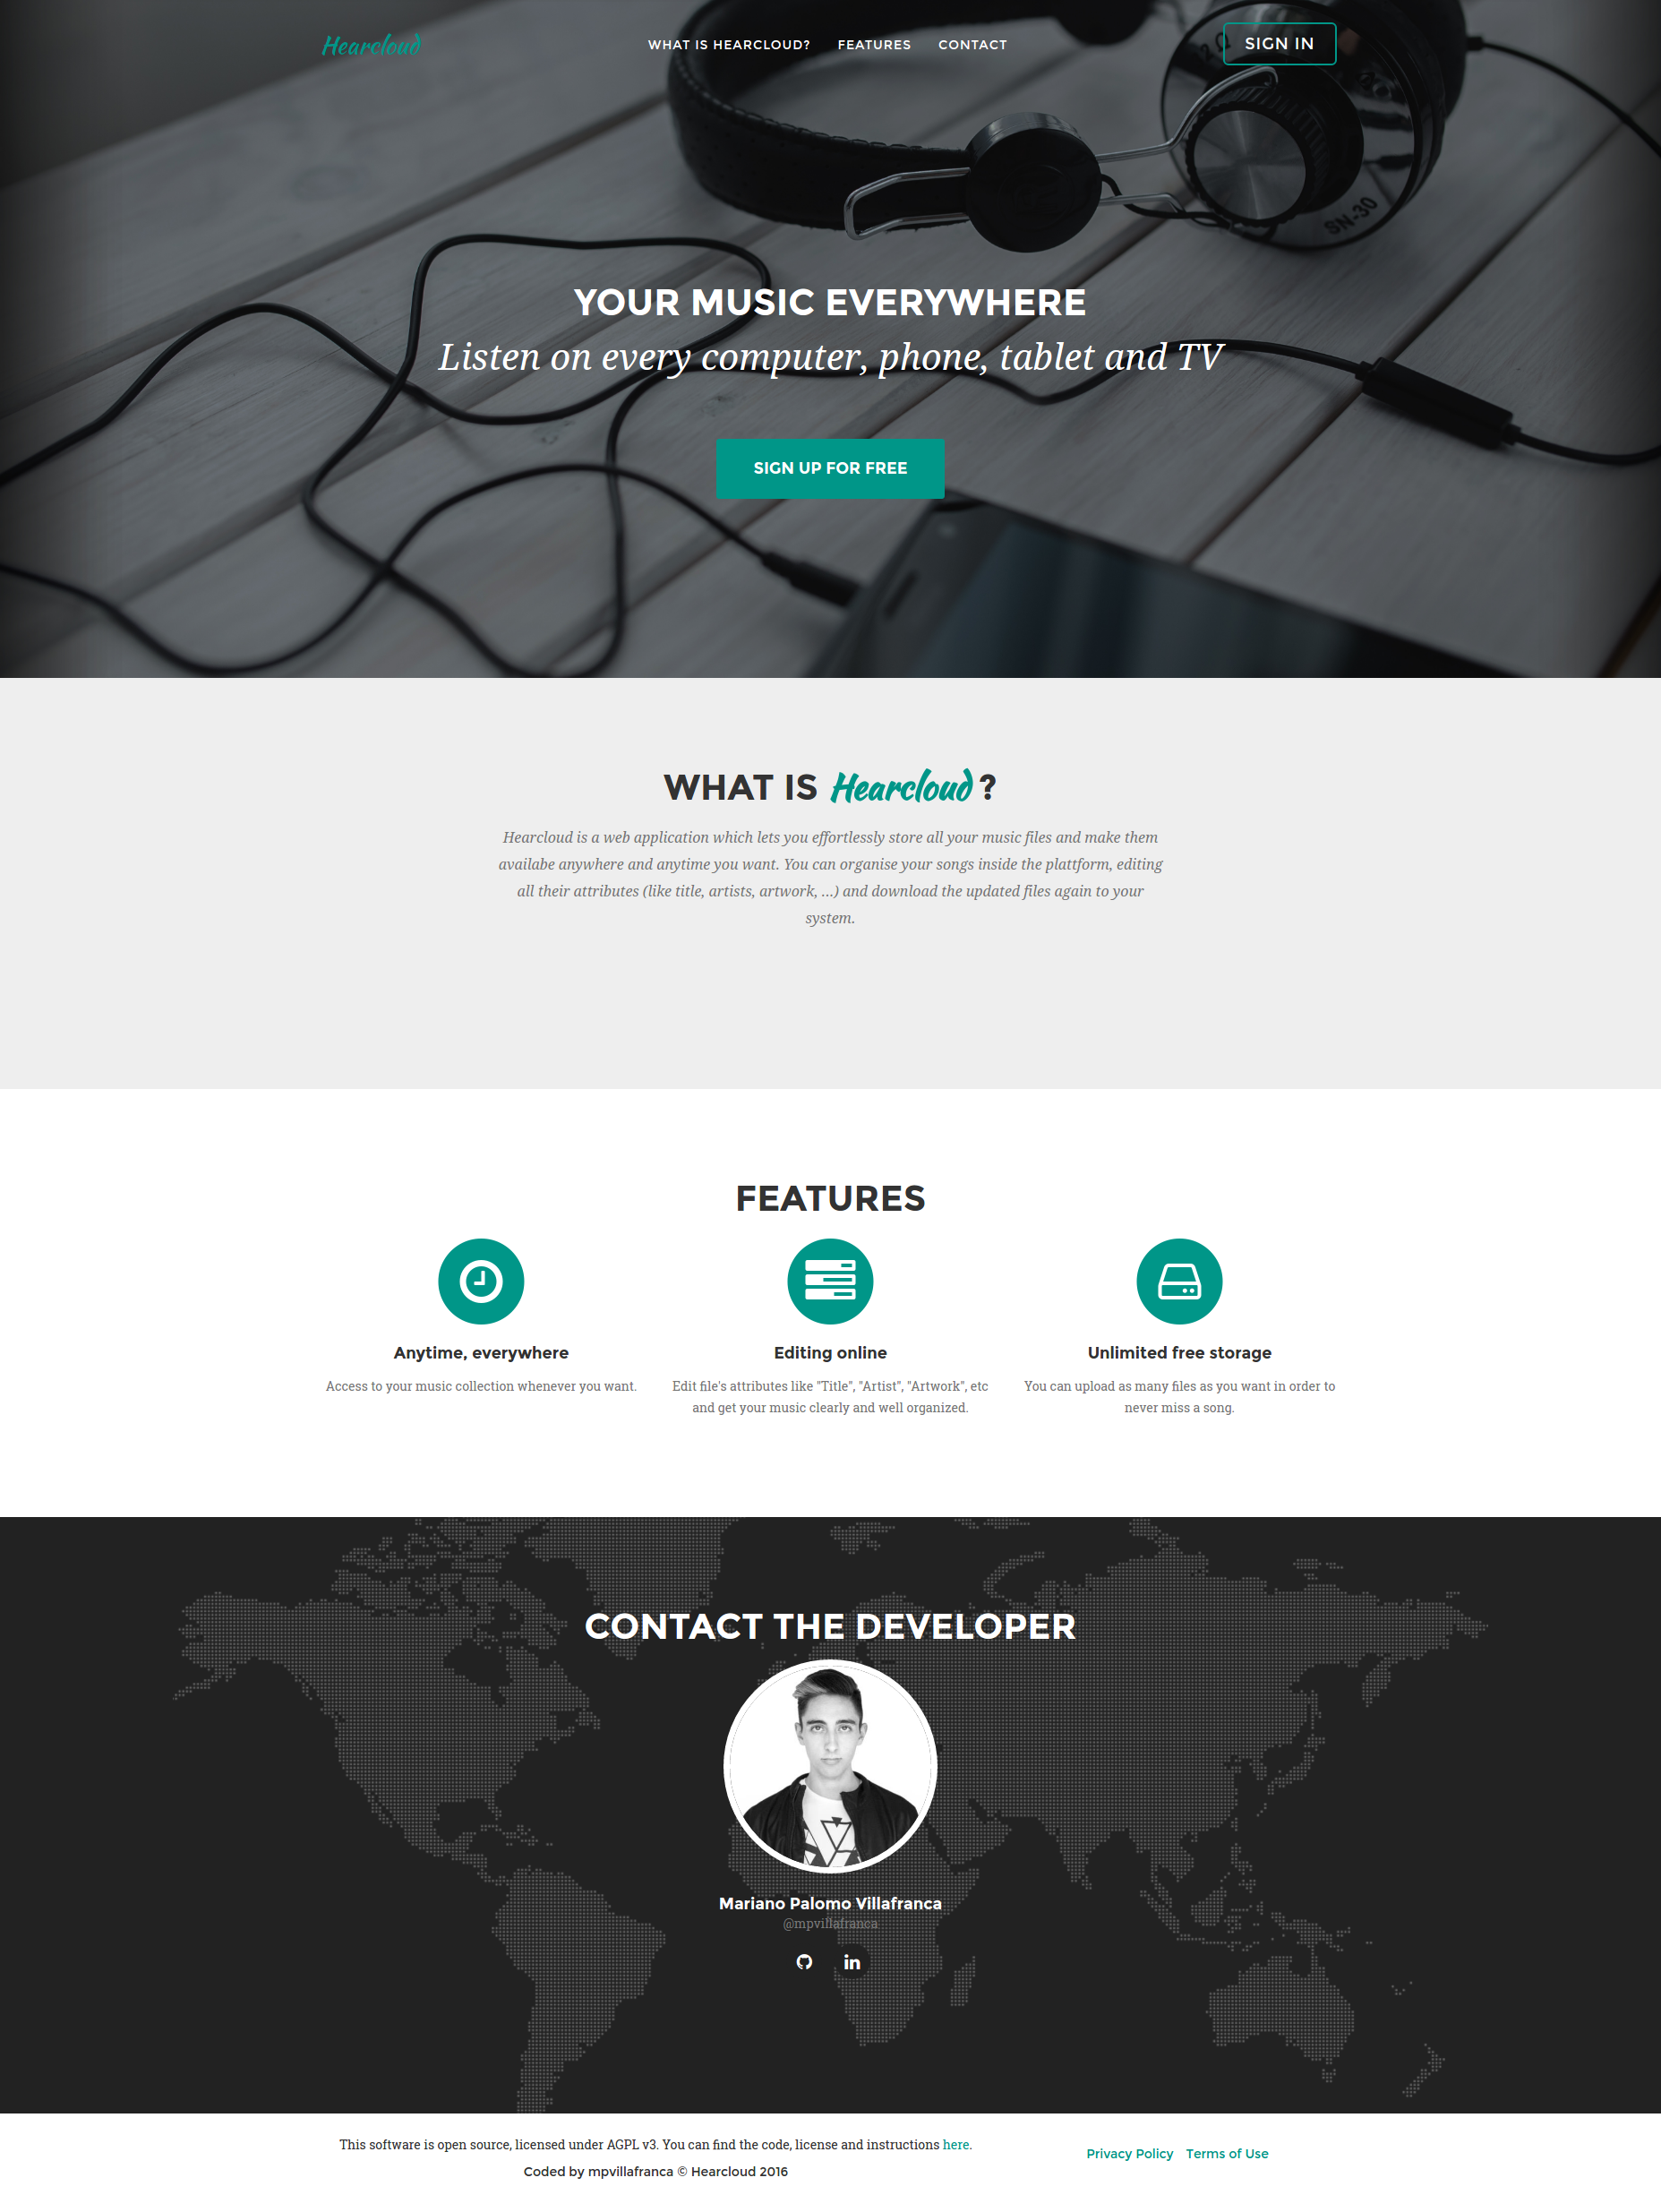
\includegraphics[scale=0.2]{../images/um/um_1.png}
\caption{Página principal (usuario no autenticado)}
\end{figure}

\subsection{Registro y acceso al sistema de usuarios}

La página de registro consiste en un formulario en el que se le solicita al usuario que introduzca un nombre de usuario, un email y una contraseña. Además, se le da la opción de cancelar el registro (lo que le redireccionaría de vuelta a la página principal) o de iniciar sesión (si ya estuviera registrado en el sistema).

\begin{figure}[H] 
\centering 
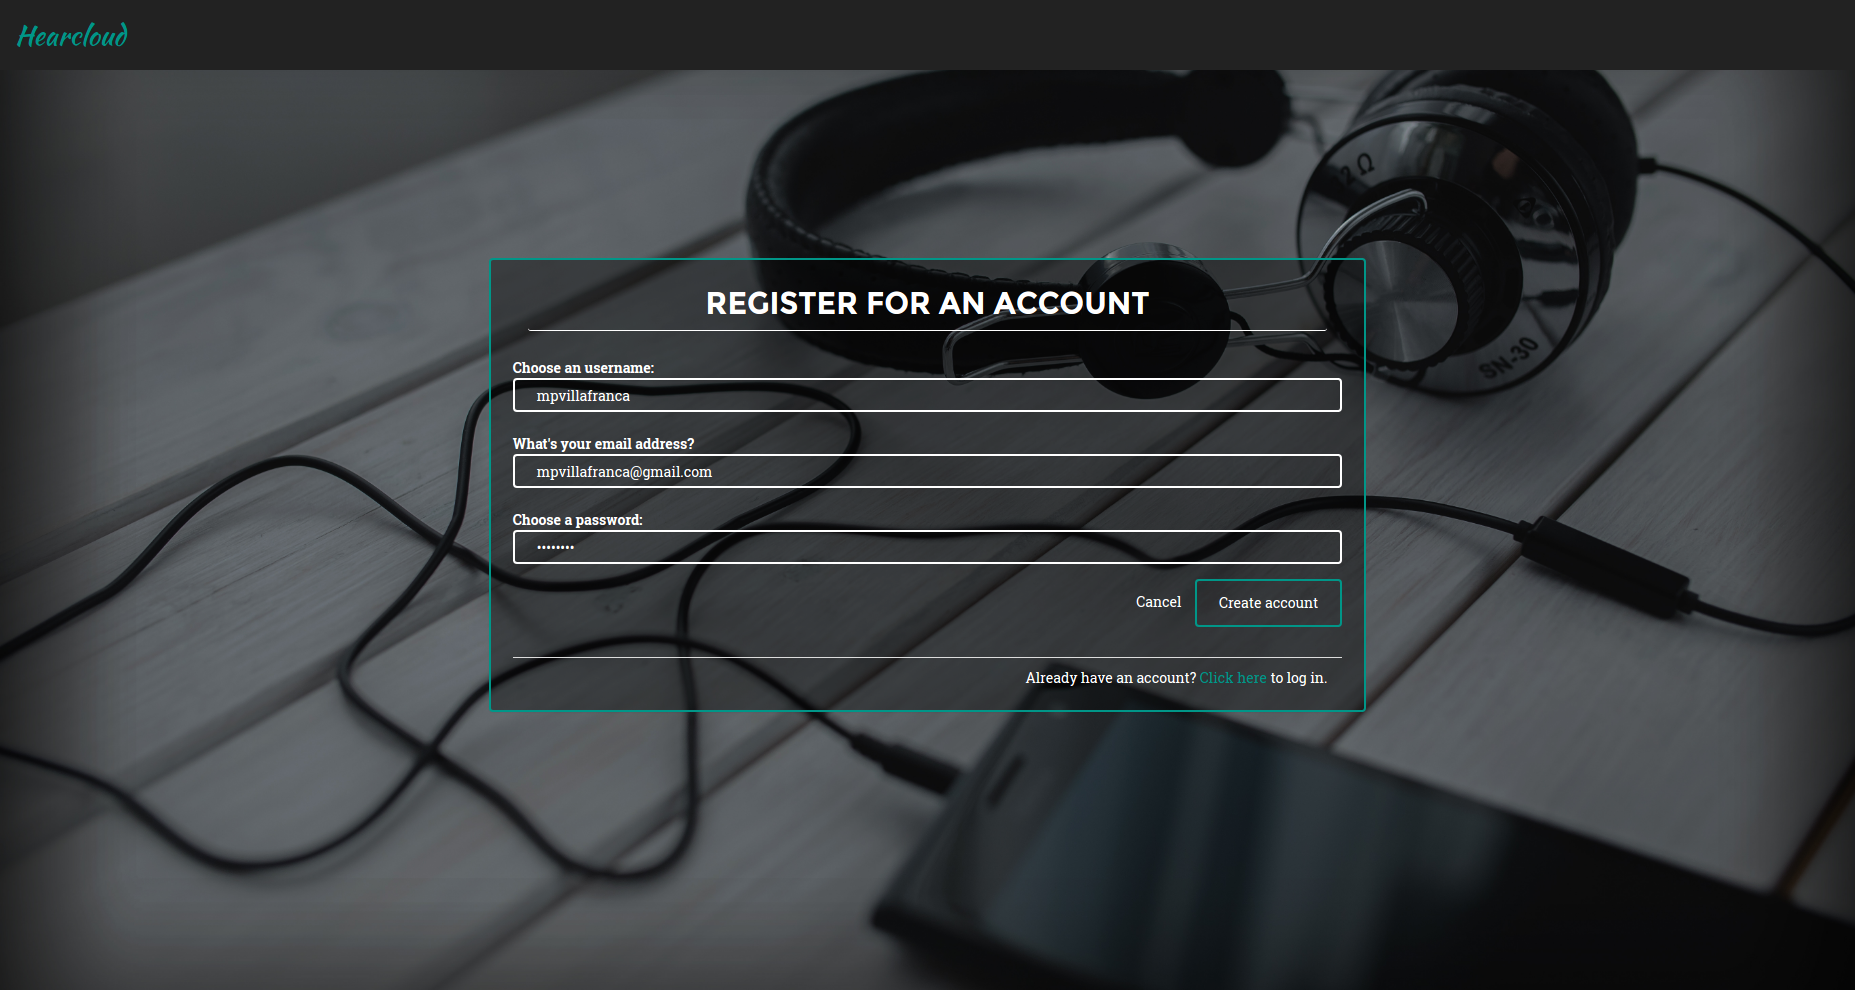
\includegraphics[scale=0.2]{../images/um/um_2.png}
\caption{Página de registro de usuarios}
\end{figure}

Al igual que en el caso anterior, la página de inicio de sesión, en la que se muestra un formulario para introducir nombre de usuario y contraseña, da la posibilidad de cancelar el inicio o de acceder al formulario de registro.

\begin{figure}[H] 
\centering 
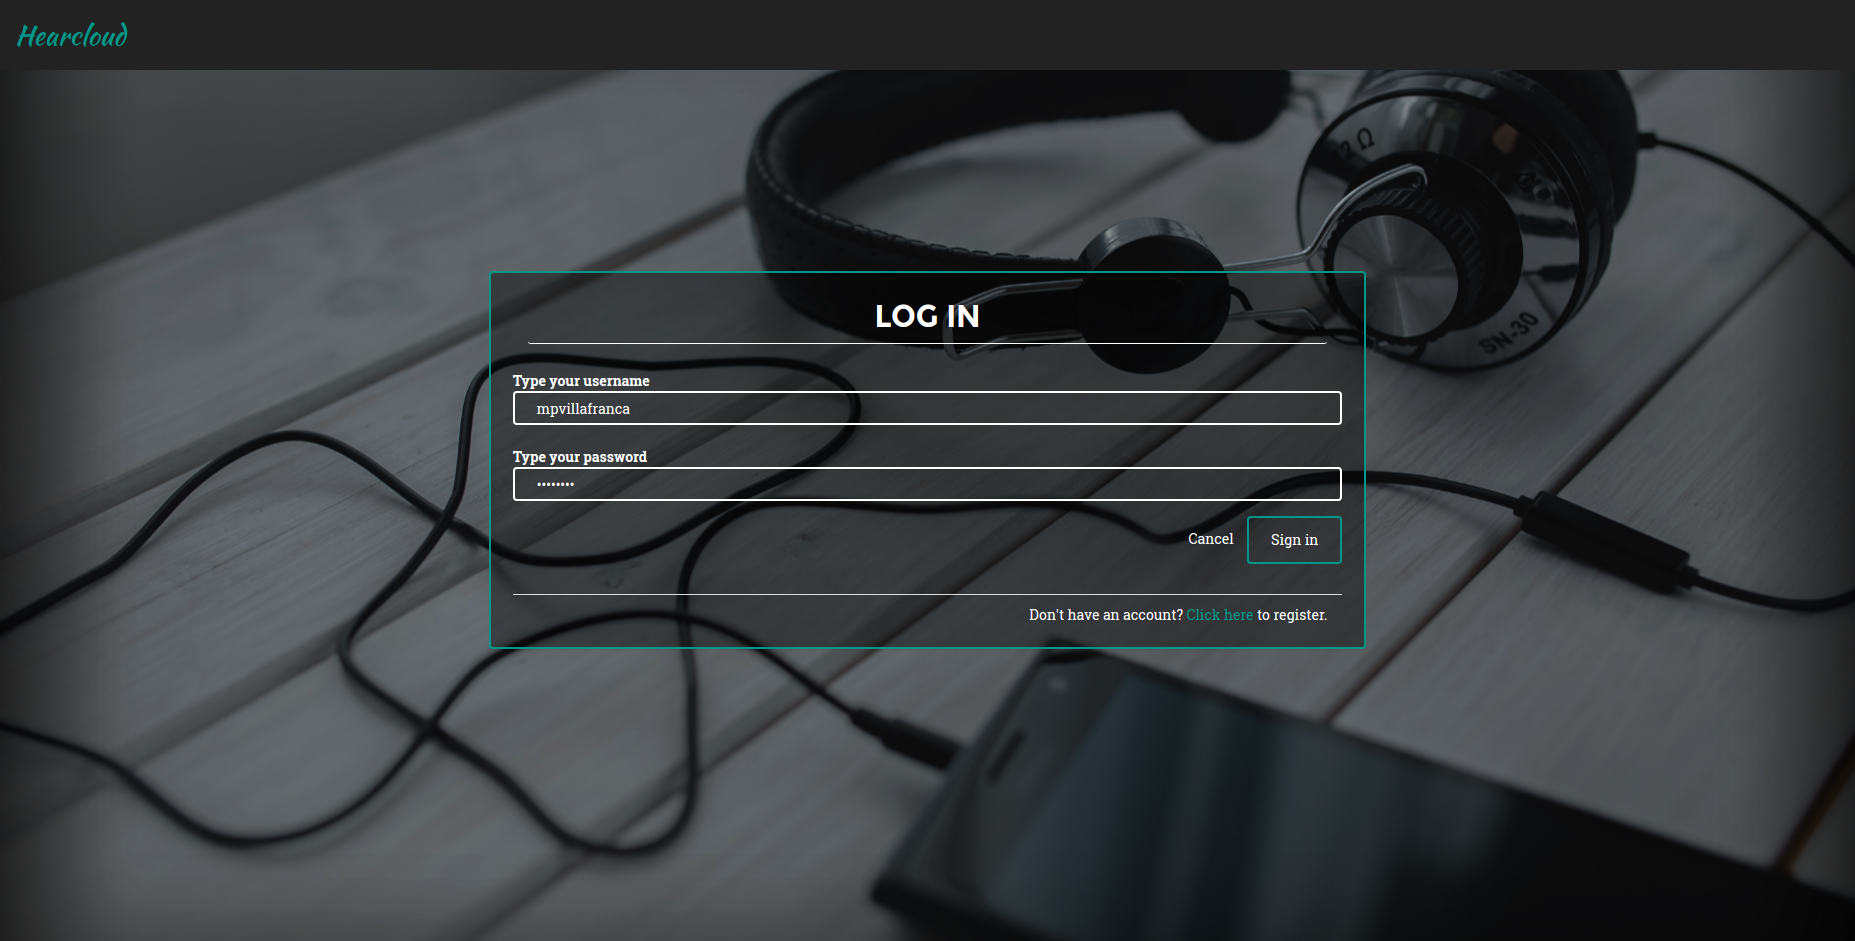
\includegraphics[scale=0.2]{../images/um/um_3.png}
\caption{Página de inicio de sesión de usuarios}
\end{figure}

\subsection{Panel principal del sistema: Canciones}

Es la vista principal del sistema para los usuarios que han iniciado sesión en la plataforma. Si es la primera vez que acceden, el panel central se mostrará vacío. Las canciones que el usuario vaya subiendo irán apareciendo en dicho panel, donde se muestra información básica acerca de la canción (imagen, título, artista, album, duración y fechas de subida y modificación). Por cada canción, aparecen tres acciones posibles a realizar en forma de botones: reproducir, descargar y eliminar.

Si se hace click en el botón de reproducir, se abrirá el reproductor integrado dentro del sistema, donde se muestran título y artista de la canción, junto a su portada y forma de onda. Además, nos podremos desplazar a lo largo de la canción para adelantarla o atrasarla. Se proporciona, por último, un boton que permite pausar la reproducción y reanudarla de nuevo en el punto en que se quedó.

Por otra parte, se ofrece la posibilidad al usuario de descargar el fichero de audio de vuelta a su sistema local, dándole la opción de realizar una conversión a otro formato de audio. Si la canción ha sido subida en un formato sin compresión (wav o aiff), las opciones de descarga serán cualquiera de los cuatro formatos disponibles (wav, aiff, m4a y mp3). Si la canción se subió en un formato con compresión (m4a y mp3), solo se podrán realizar conversiones entre dichos formatos.

\begin{figure}[H] 
\centering 
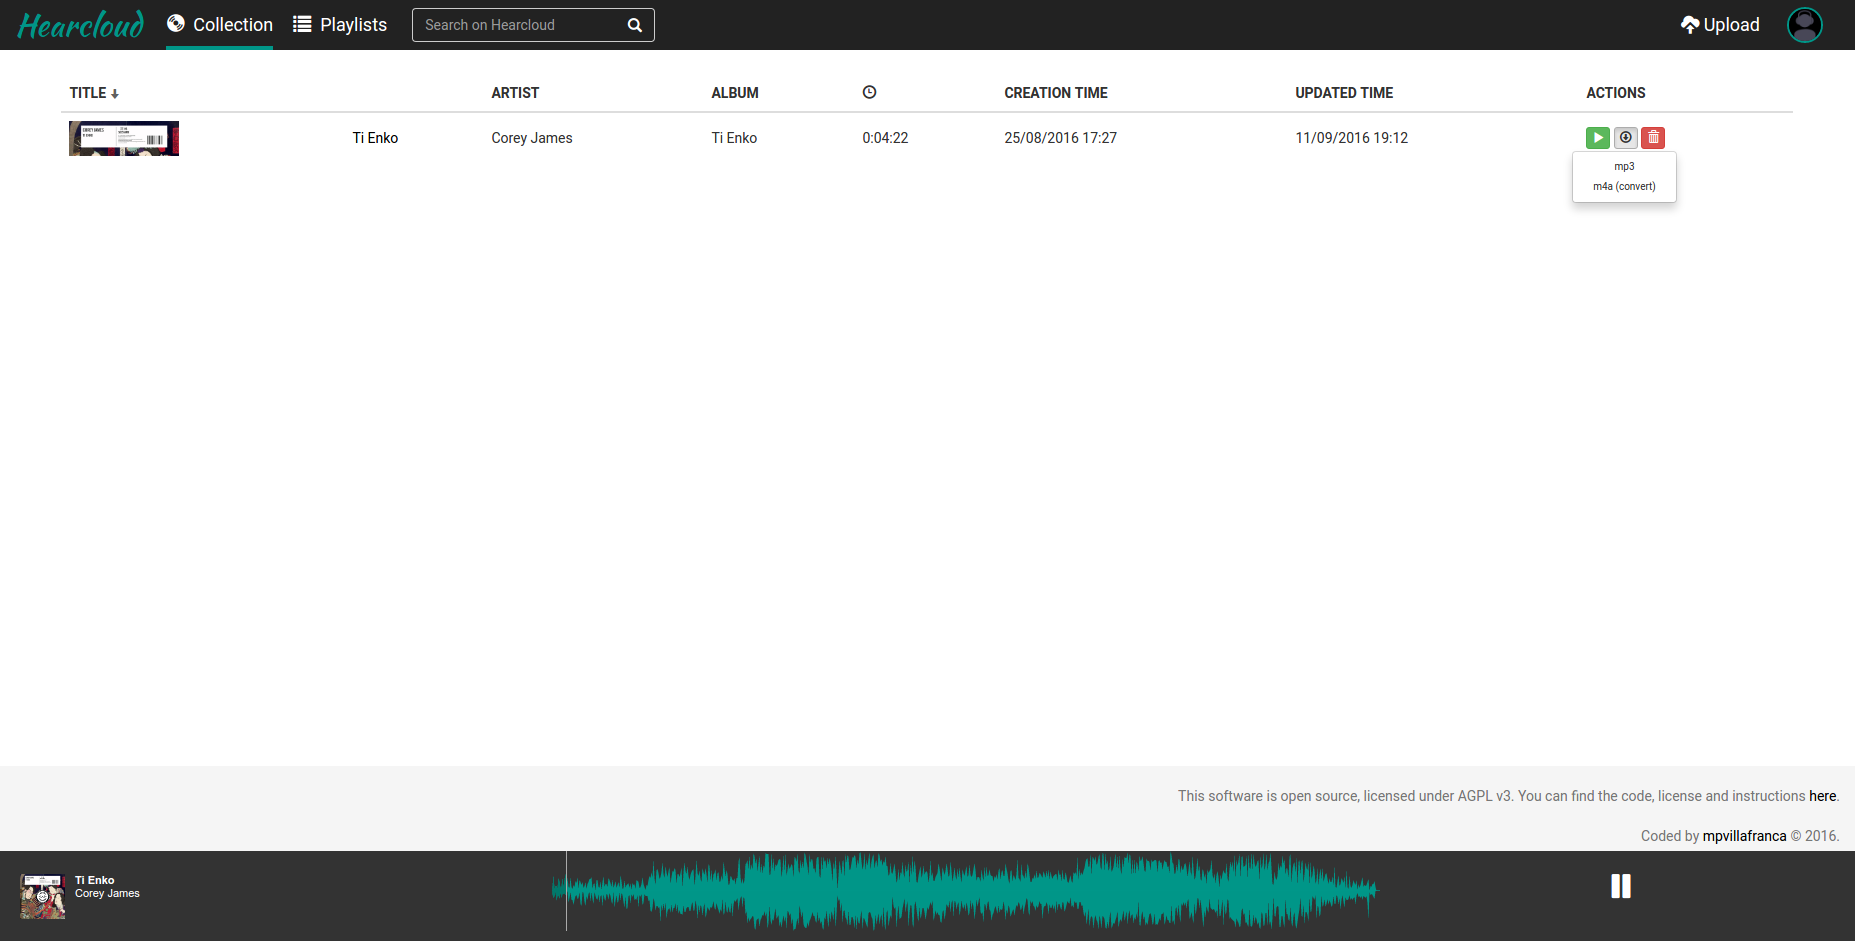
\includegraphics[scale=0.2]{../images/um/um_4.png}
\caption{Página principal (usuario autenticado)}
\end{figure}

Además, el usuario puede acceder a los detalles de la canción haciendo click en ella. En esta nueva ventana, se muestran todos los metadatos de la canción y se ofrece la posibilidad de editarlos mediante el correspondiente botón. Además, se vuelven a mostrar las opciones de reproducción, descarga y eliminación anteriores, cuyo comportamiento es idéntico al descrito anteriormente.

\begin{figure}[H] 
\centering 
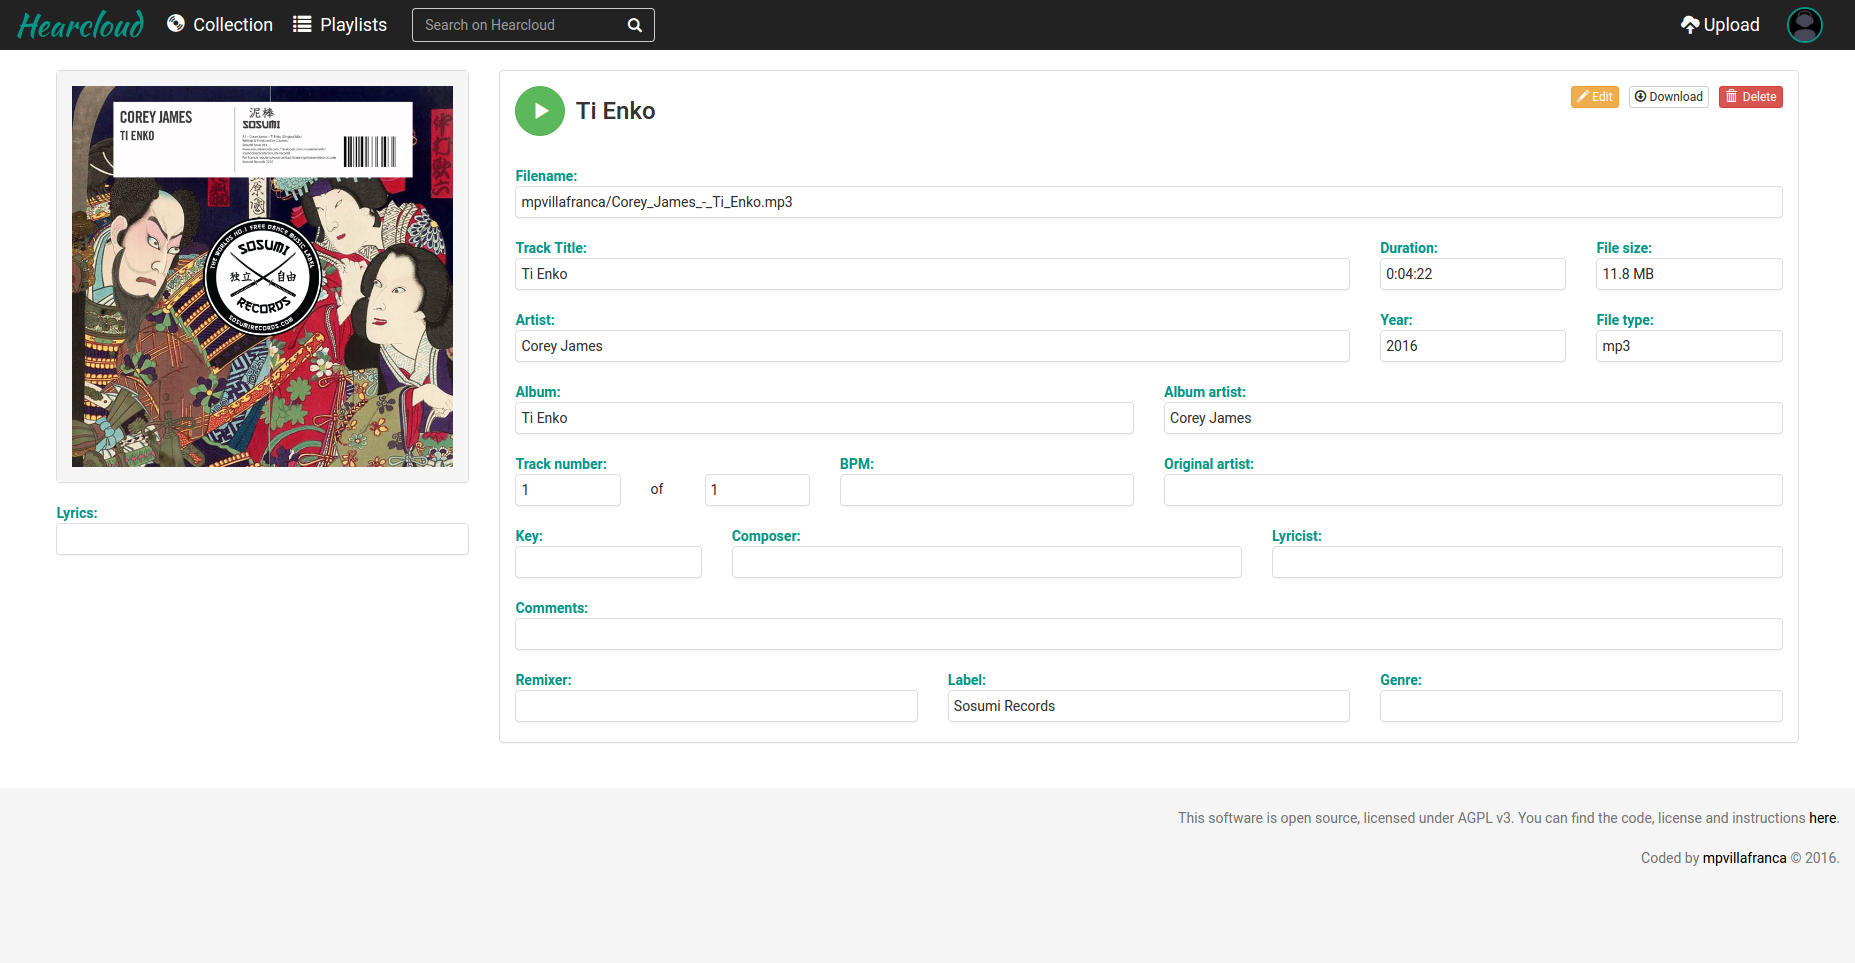
\includegraphics[scale=0.2]{../images/um/um_5.png}
\caption{Página del detalle de una canción}
\end{figure}

\subsection{Subida de ficheros}

Esta página es accesible mediante el botón \textit{Upload} situado en la barra de navegación del sistema. En ella, se da la posibilidad al usuario de subir a la plataforma cuantas canciones desee en una sola vez, aunque también puede seleccionar subir únicamente determinadas canciones de todas las seleccionadas inicialmente. Además, se ha implementado una \textit{drop zone}, donde el usuario puede arrastrar las canciones directamente desde el sistema sin necesidad de pulsar sobre el botón \texttt{Add files}.

\begin{figure}[H] 
\centering 
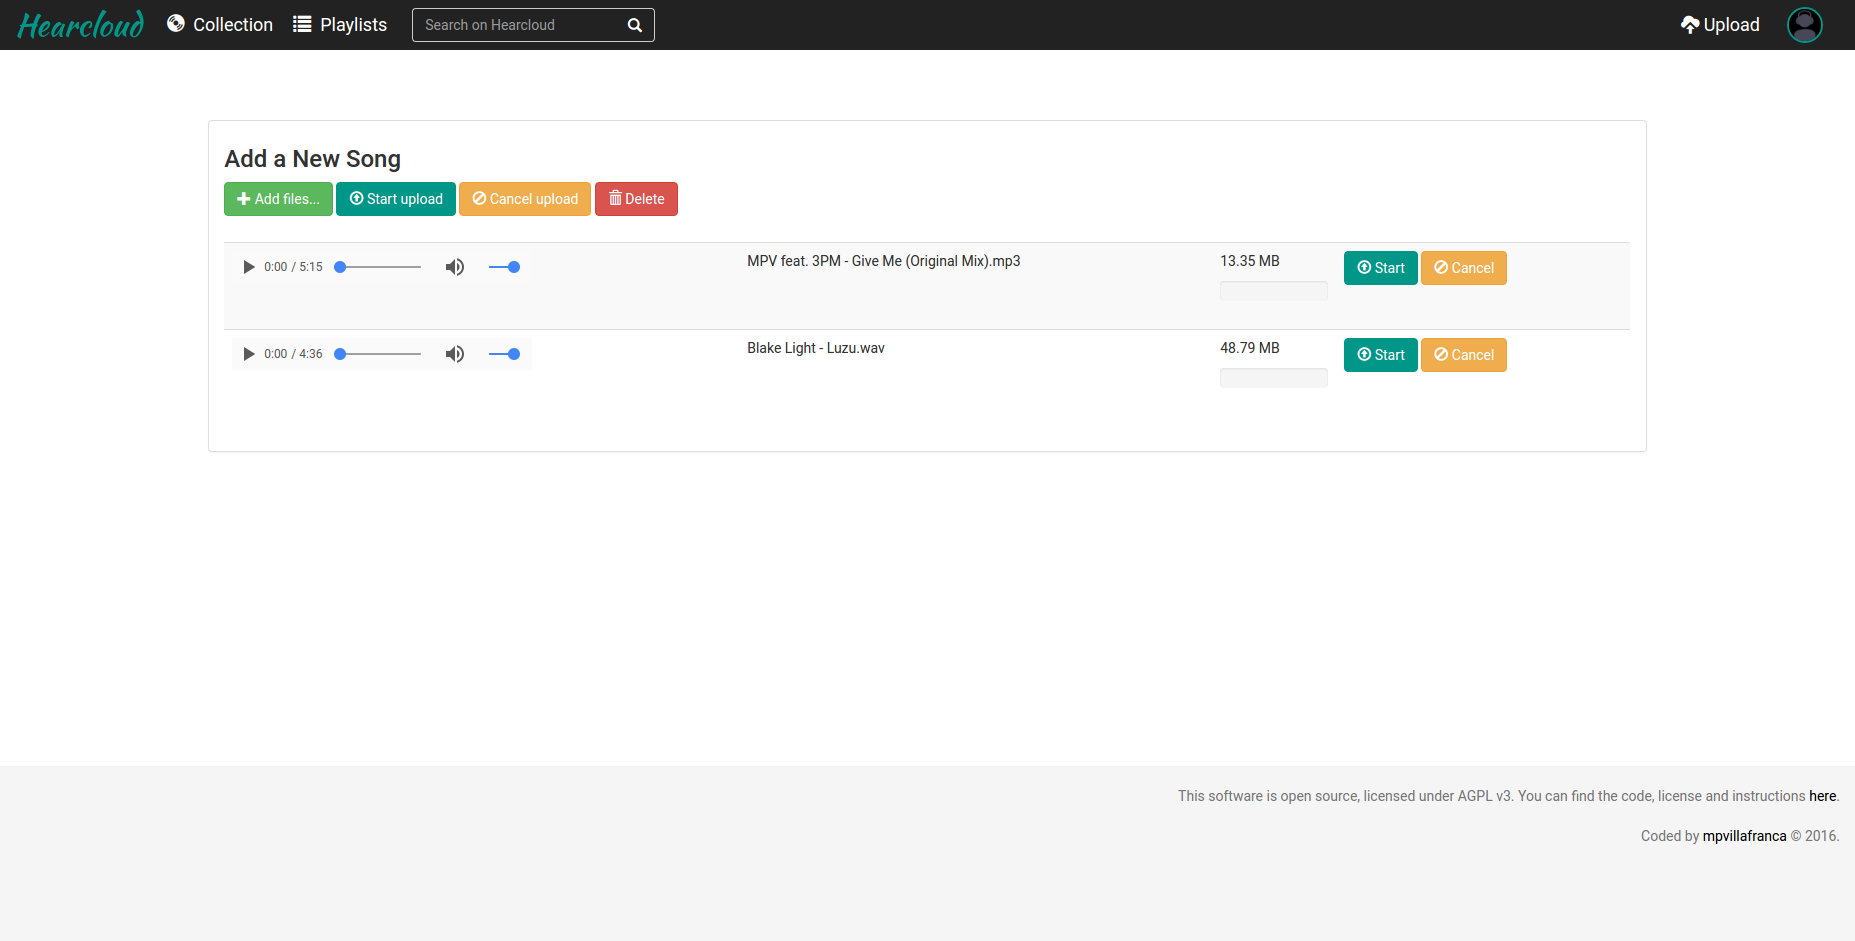
\includegraphics[scale=0.2]{../images/um/um_6.png}
\caption{Página de subida de canciones}
\end{figure}

\subsection{Panel perfil de usuario}

Este panel es accesible a través de la imagen de perfil del usuario situada en el borde superior derecho de la barra de navegación. En ella, se muestra la imagen de perfil del usuario, sus datos básicos y un contador sobre el número de canciones y listas de reproducción que tiene en su sistema.

\begin{figure}[H] 
\centering 
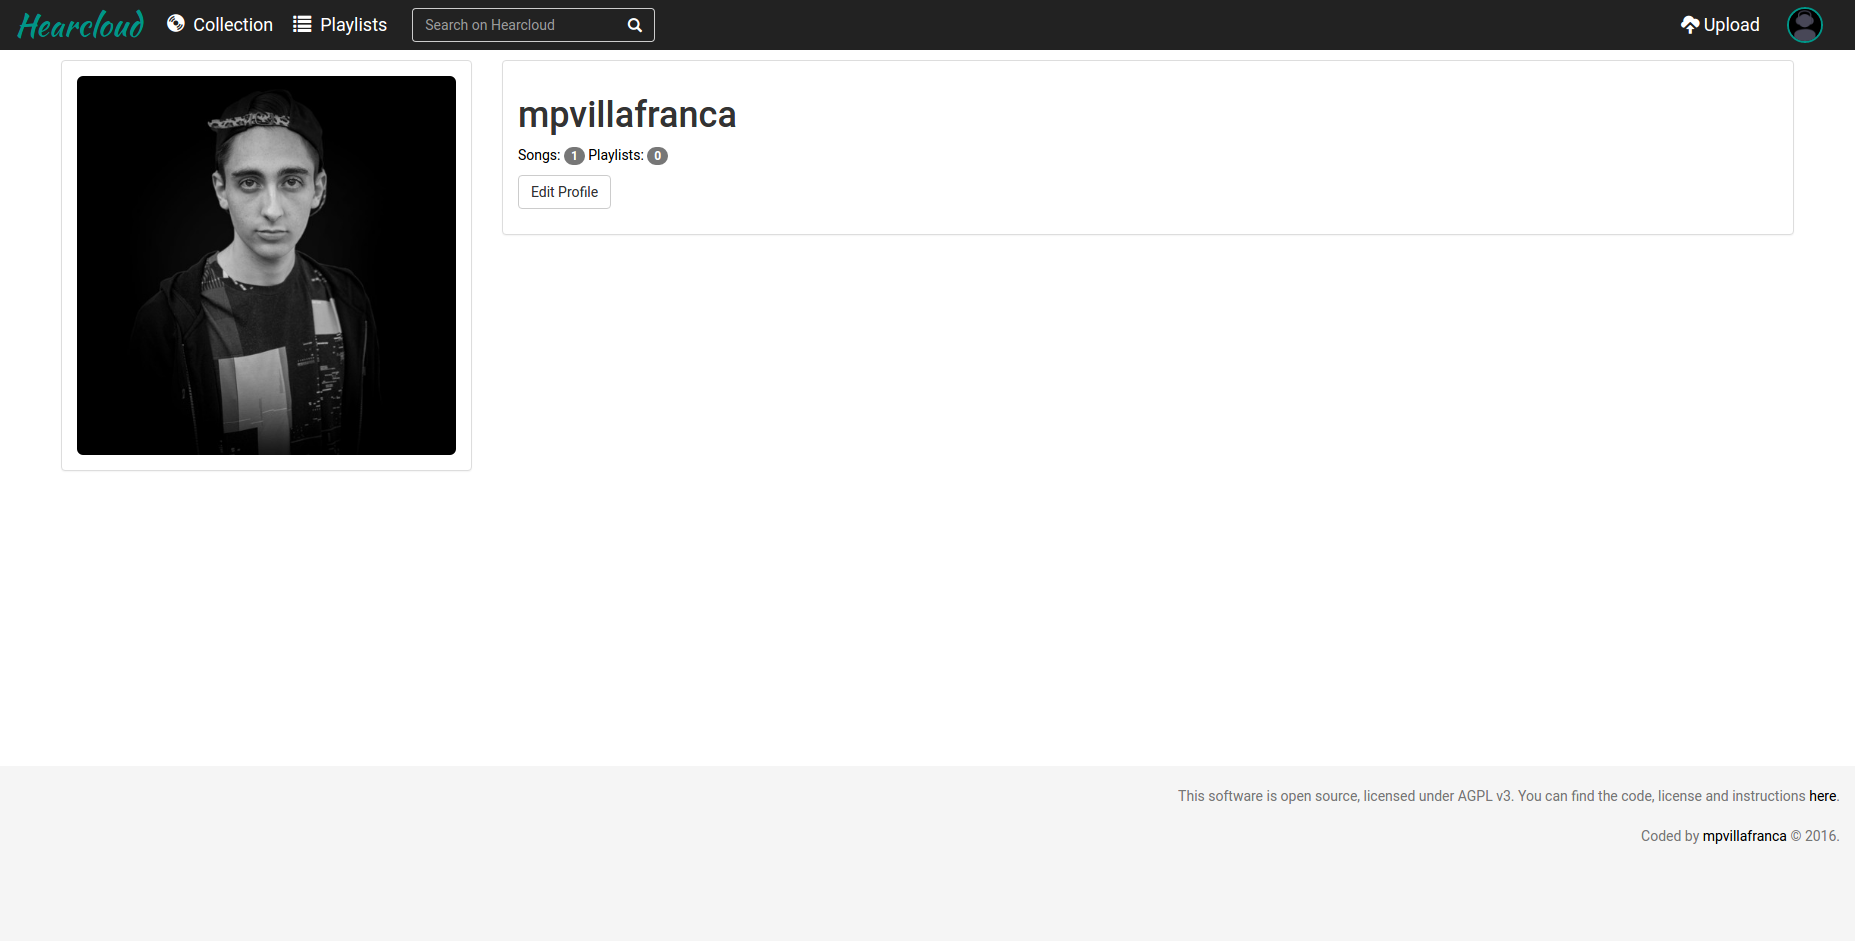
\includegraphics[scale=0.2]{../images/um/um_7.png}
\caption{Página del perfil de usuario}
\end{figure}

\subsection{Panel de administración}

Django ofrece un panel de administración accesible a través de la url \texttt{/admin}, al que podrán acceder todos los usuarios que tengan activado el atributo \texttt{is\_staff}. Las opciones que aquí se les muestren dependerán de los permisos que se les concedan. 

\begin{figure}[H] 
\centering 
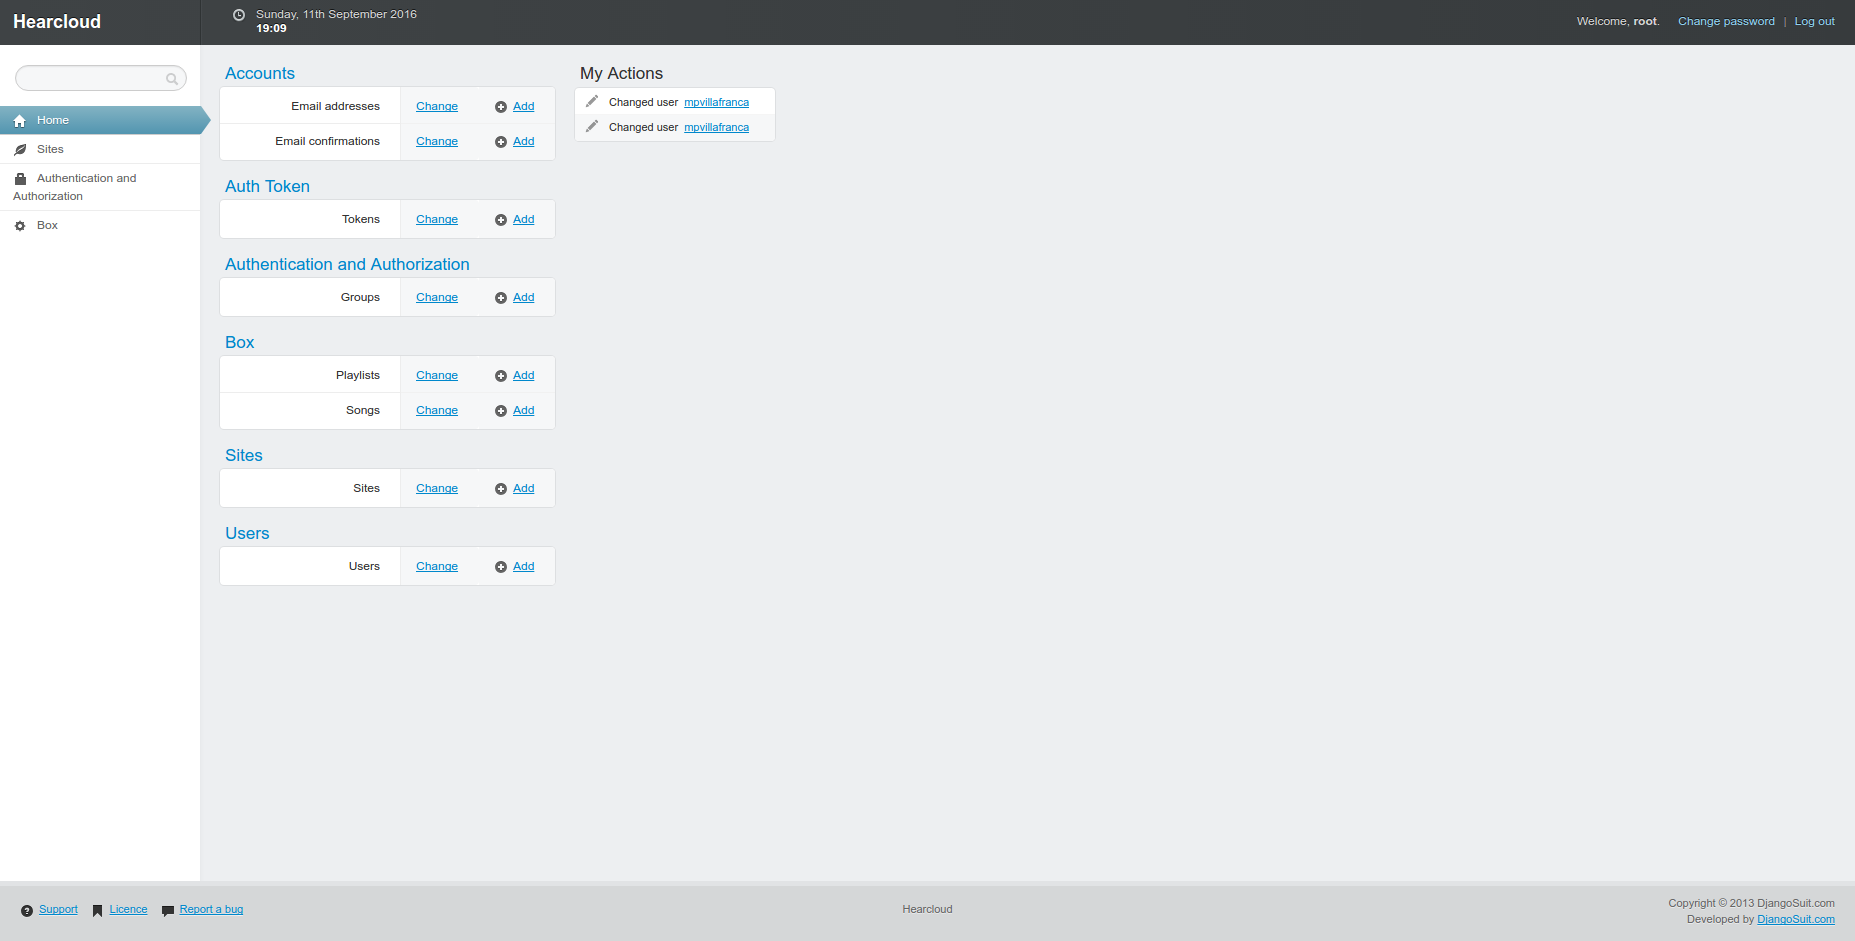
\includegraphics[scale=0.2]{../images/um/um_8.png}
\caption{Panel de administración de Django. Vista principal.}
\end{figure}

Si el usuario que accede posee todos los permisos o es superusuario, se desplegarán todas las opciones disponibles. Con él, podremos gestionar los usuarios y grupos del sistema y los ficheros y listas de reproducción que éstos almacenen.

\begin{figure}[H] 
\centering 
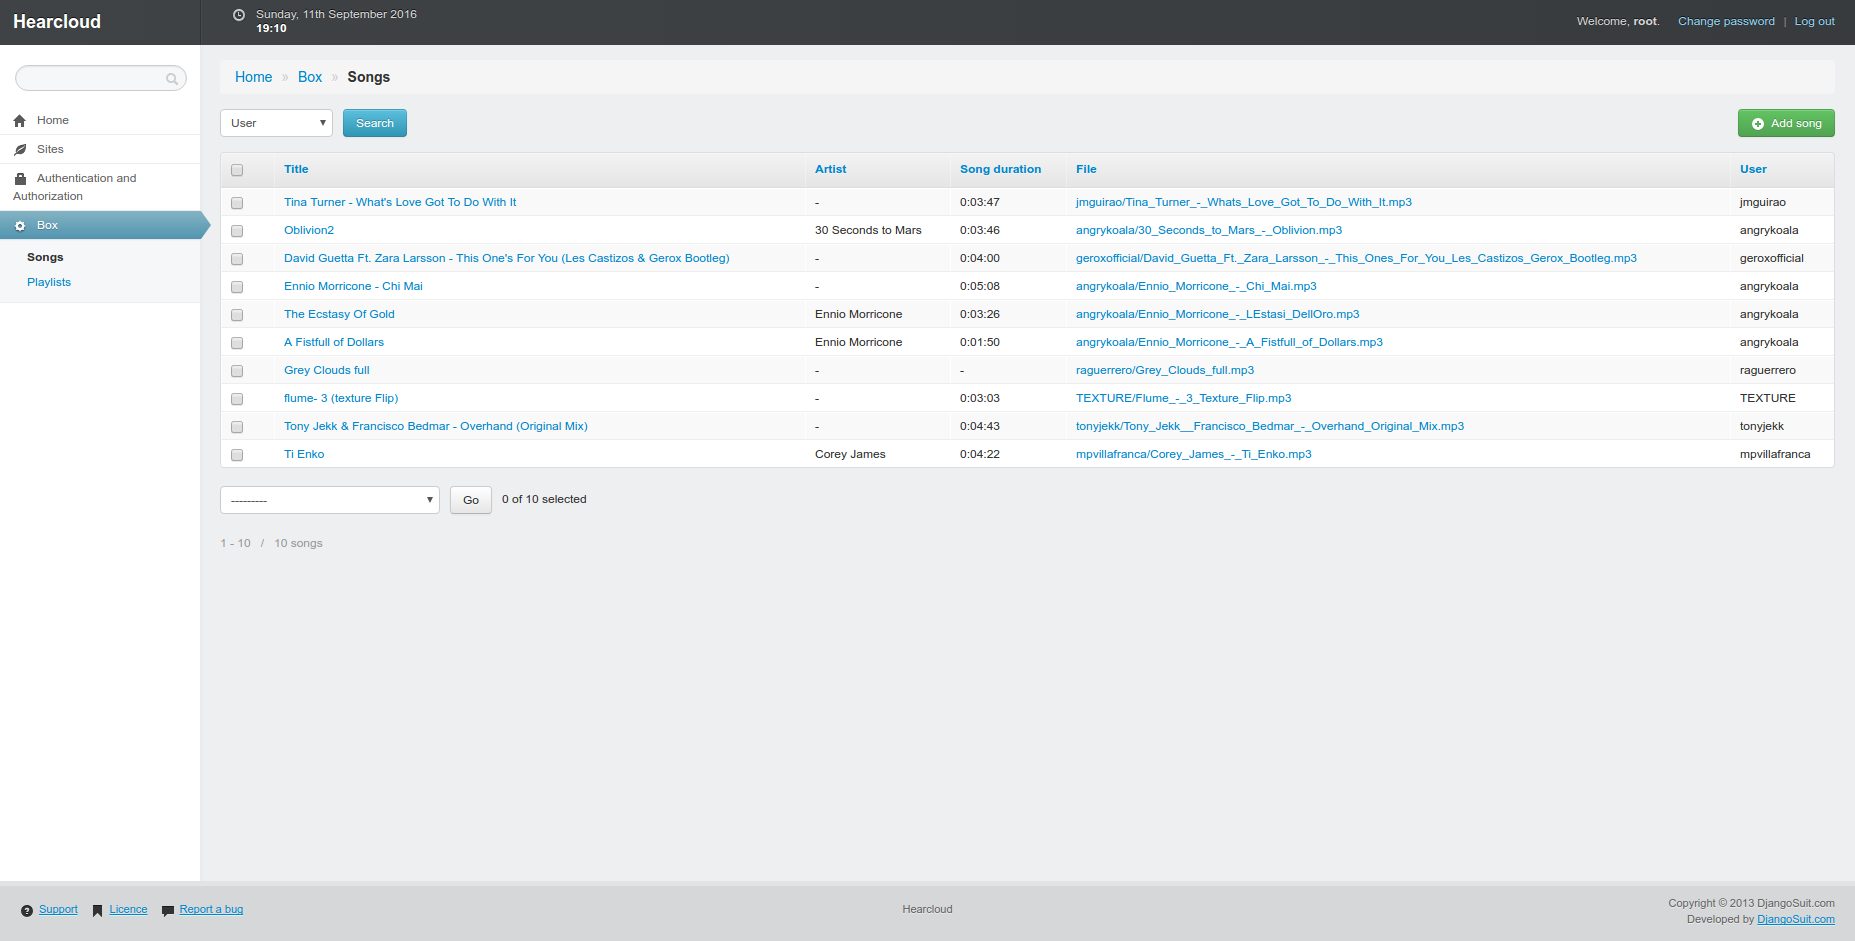
\includegraphics[scale=0.2]{../images/um/um_9.png}
\caption{Panel de administración de Django. Lista de canciones del sistema.}
\end{figure}

\subsection{Diseño adaptativo. Versión móvil}

Durante el desarrollo del sistema se ha tenido en cuenta que la plataforma se adapte lo máximo posible a los diferentes dispositivos desde los que se pueda acceder a ella, por lo que todas las secciones descritas anteriormente, deberían de visualizarse correctamente sin importar desde dónde se esté accediendo.

\begin{figure}[H]
\minipage{0.32\textwidth}
  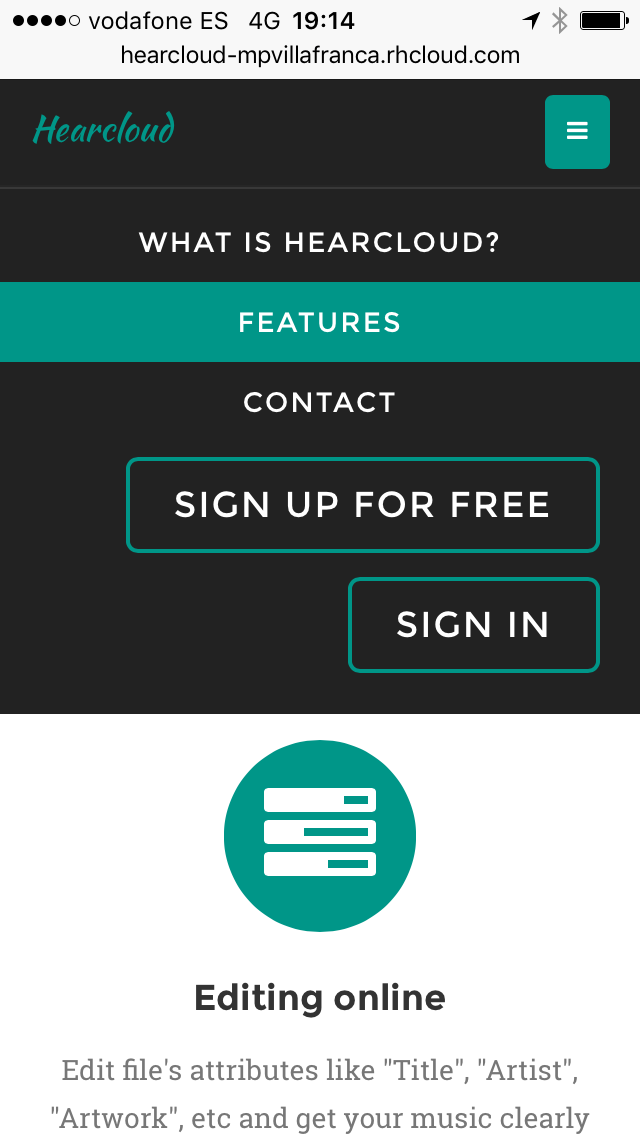
\includegraphics[width=\linewidth]{../images/um/um_10.png}
  \caption{Página principal (usuario no autenticado) en iPhone 6S}
\endminipage\hfill
\minipage{0.32\textwidth}
  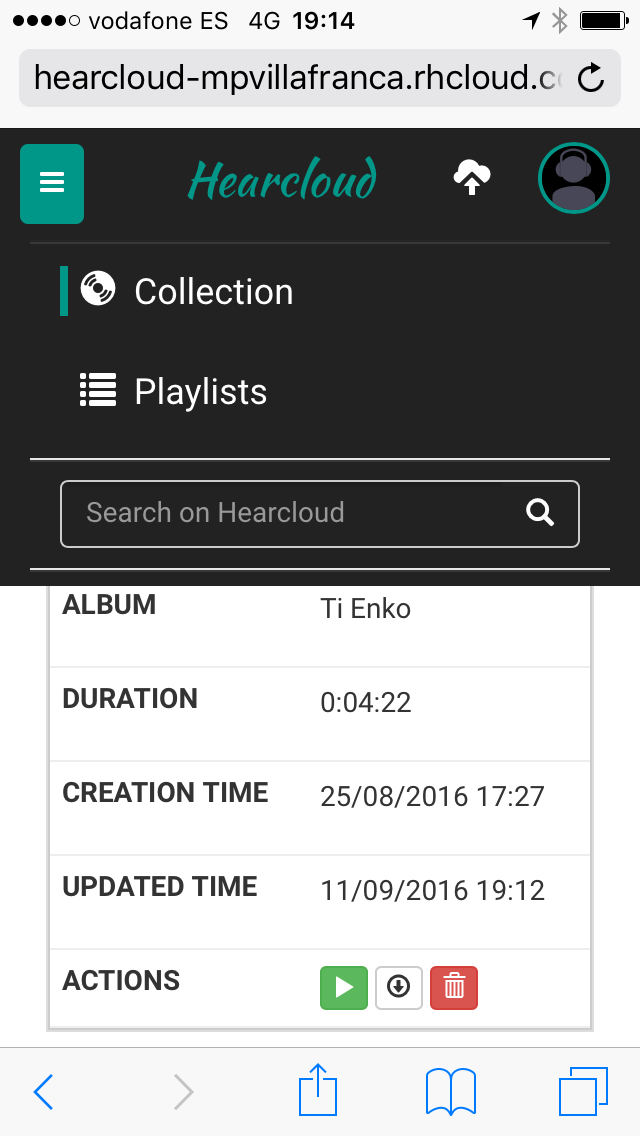
\includegraphics[width=\linewidth]{../images/um/um_11.png}
  \caption{Página principal (usuario autenticado) en iPhone 6S}
\endminipage\hfill
\end{figure}

\newpage